\documentclass{beamer}
\usetheme{metropolis}
\usepackage{appendixnumberbeamer}

\usepackage{pgfplots}

\title{From image to video understanding in machine learning}
\date{\today}
\author{Brendan Duke}
\institute{University of Guelph}

\begin{document}

\maketitle

\begin{frame}{Table of contents}
  \setbeamertemplate{section in toc}[sections numbered]
  \tableofcontents[hideallsubsections]
\end{frame}

\section{Introduction}

\begin{frame}{ActivityNet}
        \center
        
\includegraphics[scale=1.0]{data/activity-net.png}
\end{frame}

\begin{frame}[fragile]{Questions to ponder}
        \begin{itemize}[<+- | alert@+>]
                \item Do the techniques that brought success on ImageNet
                        generalize to video understanding?

                \item Can the temporal information in video be leveraged to
                        outperform techniques that work on static images?
        \end{itemize}
\end{frame}

\section{Classification}

{%
\setbeamertemplate{frame footer}{\cite{DBLP:journals/corr/RussakovskyDSKSMHKKBBF14} and~\cite{kay2017kinetics}}
\begin{frame}{Comparing classification in images and video}
        \begin{columns}[T,onlytextwidth]
                \metroset{block=fill}

                \column{0.5\textwidth}
                        \begin{block}{
\includegraphics[scale=0.15]{data/imagenet.png}}
                                \begin{itemize}
                                        \item 1 431 167 annotated images.
                                        \item ``Trimmed'' version of entire ImageNet, which covers all English nouns.
                                        \item 1000 classes, 90 of which are dog breeds.
                                        \item $1:1$ ratio of labels to images.
                                \end{itemize}
                        \end{block}
                \column{0.5\textwidth}
                        \begin{block}{Kinetics}
                                \begin{itemize}
                                        \item 306 245 annotated 10s video clips.
                                        \item Human actions: e.g.\ hugging, washing dishes.
                                        \item 400 classes.
                                        \item $\approx 1:100$ ratio of labels to RGB frames, assuming 10fps on average.
                                \end{itemize}
                        \end{block}
        \end{columns}
\end{frame}
}

{%
\setbeamertemplate{frame footer}{Image:~\url{https://research.googleblog.com}}
\begin{frame}{Image classification architecture: Inception-ResNet-v2}
        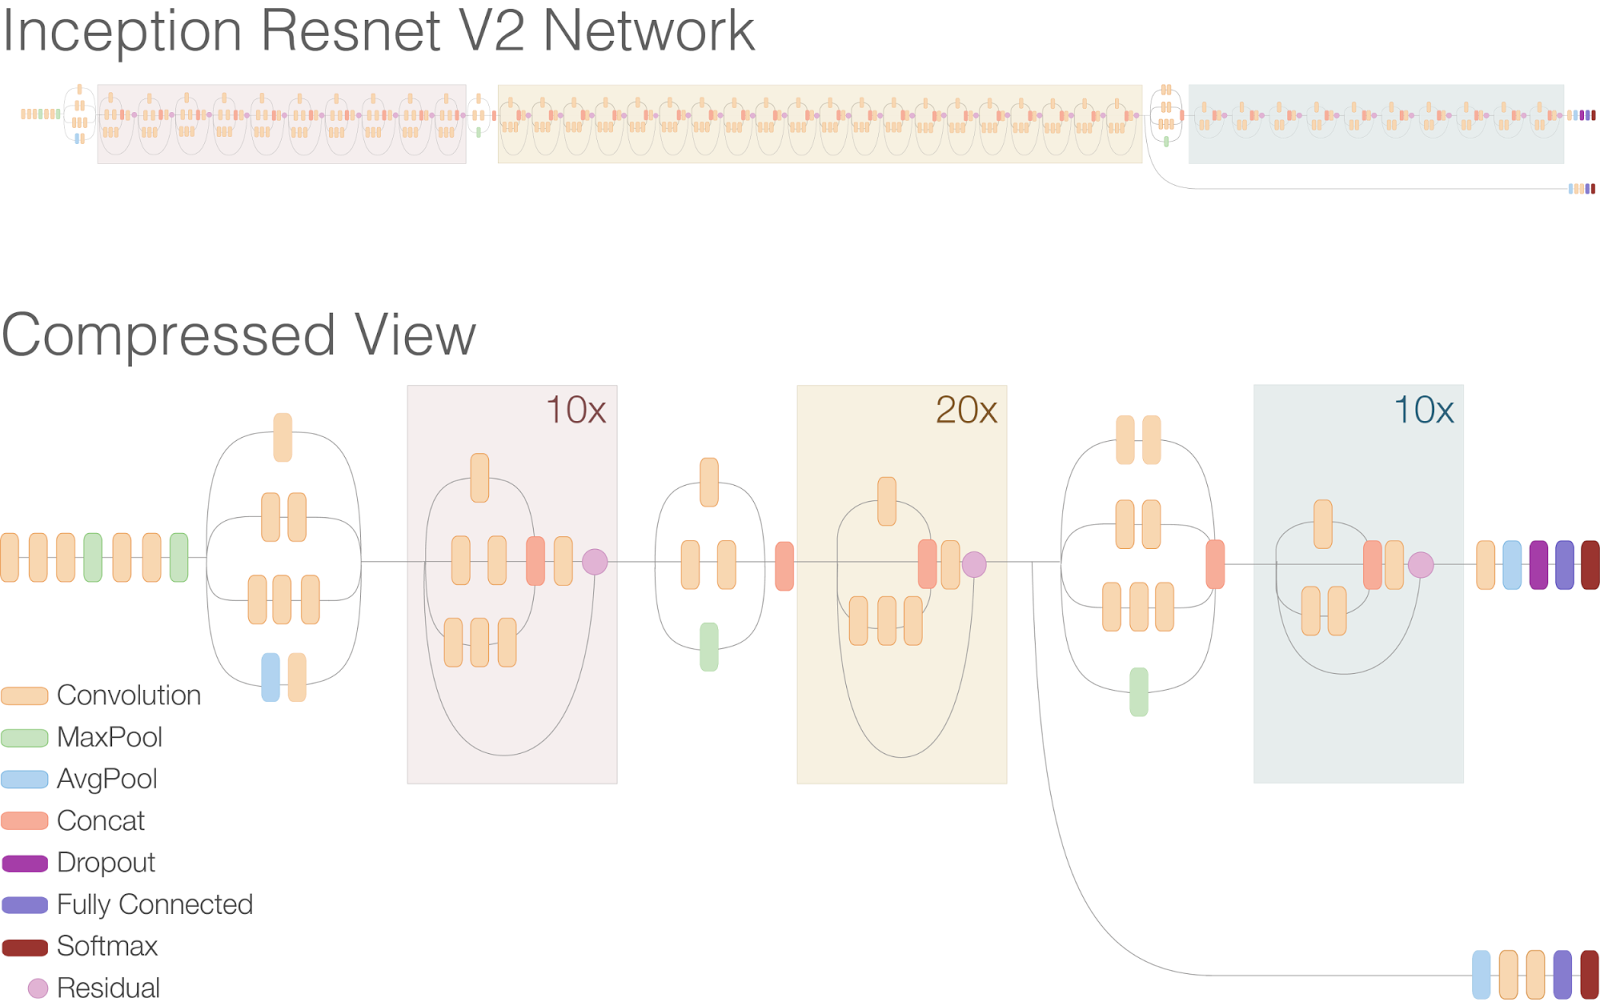
\includegraphics[scale=0.2]{data/inception-resnet-v2.png}
\end{frame}
}

{%
\setbeamertemplate{frame footer}{Image:~\cite{carreira2017quo}}
\begin{frame}{Video classification architectures}
        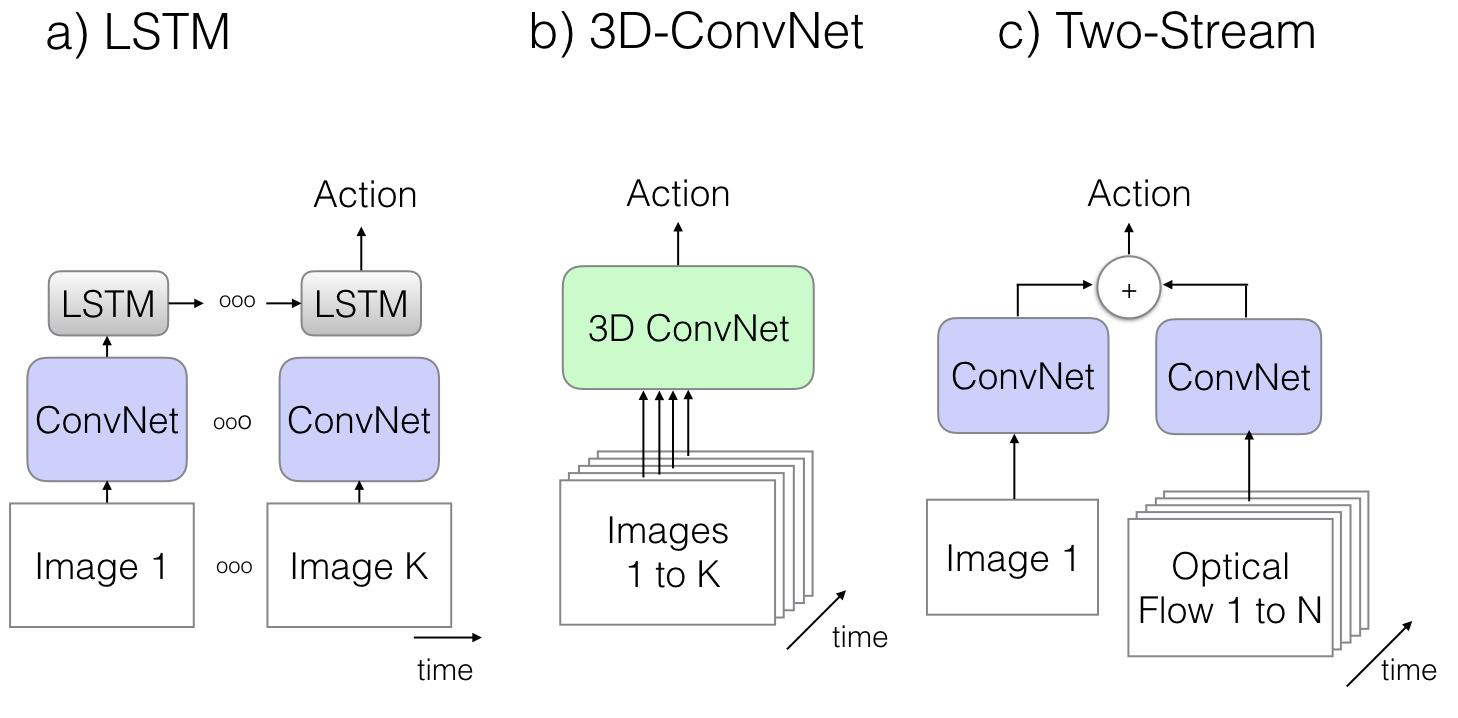
\includegraphics[scale=0.22]{data/lstm-3d-convnet-two-stream-cropped.png}
\end{frame}
}

{%
\setbeamertemplate{frame footer}{Image:~\cite{DBLP:journals/corr/SimonyanZ14a}}
\begin{frame}{Optical flow}
        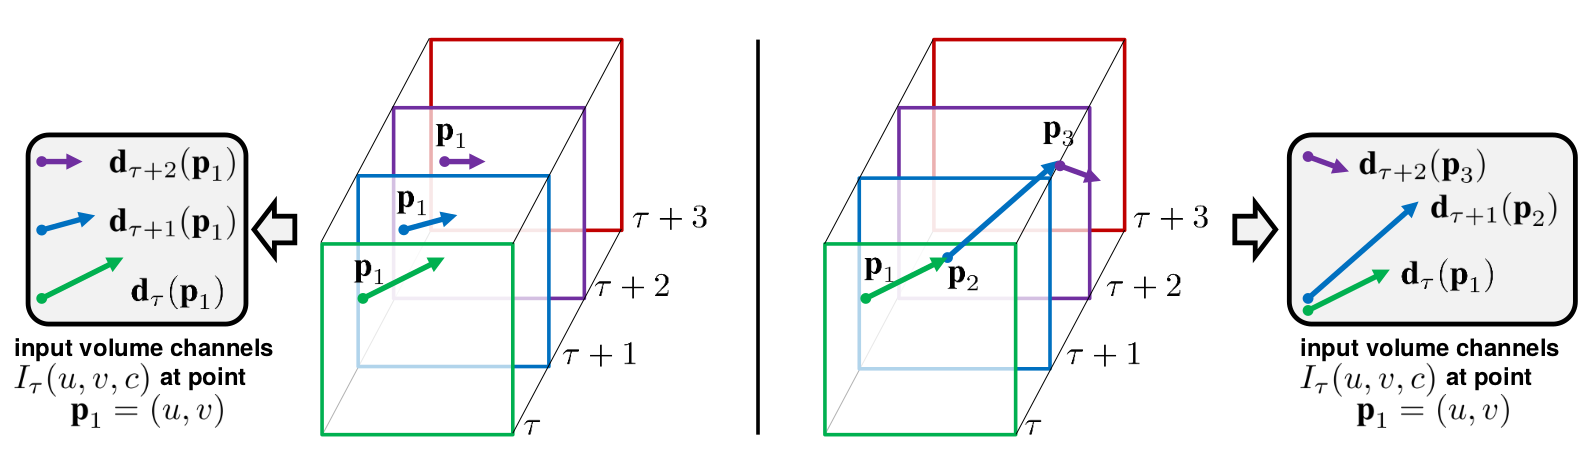
\includegraphics[scale=0.2]{data/optical-flow-vectors.png}
\end{frame}
}

,
                                width=0.9\textwidth,
                                height=6cm,
                                xtick=data,
                                xticklabels={RGB, Flow, RGB \& Flow},
                                y filter/.expression={y==0 ? nan : y},
                                ymin=0
                        ]

                                \addplot plot coordinates {(0, 25.9) (1, 30.4) (2, 21.3)};
                                \addplot plot coordinates {(0, 29.9) (1, 41.6) (2, 27.1)};
                                \addplot plot coordinates {(0, 30.1) (1, 0) (2, 0)};
                                \addplot plot coordinates {(0, 40.0) (1, 0) (2, 0)};

                                \legend{Two-Stream I3D, Two-Stream, LSTM, 3D-ConvNet}

                        \end{axis}
                \end{tikzpicture}
        \end{figure}
\end{frame}
}

\section{Detection}

{%
\setbeamertemplate{frame footer}{Image: \cite{DBLP:journals/corr/RenHG015}}
\begin{frame}{Faster R-CNN}
        \center
        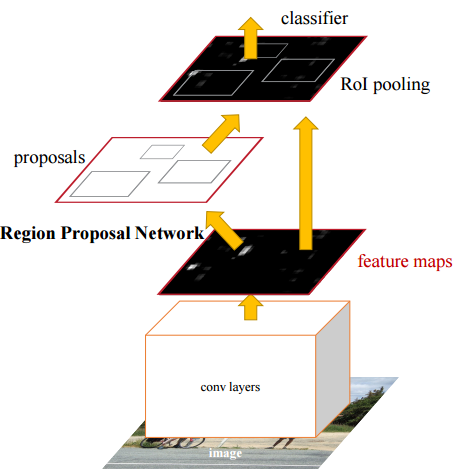
\includegraphics[scale=0.55]{data/faster-rcnn.png}
\end{frame}
}

{%
\setbeamertemplate{frame footer}{Image: \cite{DBLP:journals/corr/KangLXOYLW17}}
\begin{frame}{Tubelet proposal networks}
        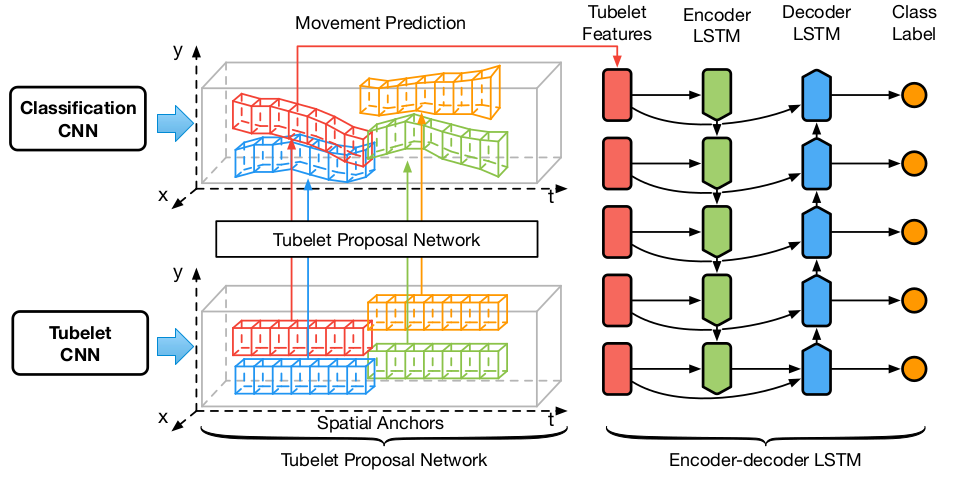
\includegraphics[scale=0.3]{data/tubelet-proposal-network.png}
\end{frame}
}

{%
\setbeamertemplate{frame footer}{\cite{DBLP:journals/corr/KangLXOYLW17}}
\begin{frame}{ImageNet VID results}
        \begin{figure}
                \begin{tikzpicture}
                        \begin{axis}[
                                        mbarplot,
                                xlabel={Method},
                                ylabel={Mean AP},
                                width=0.9\textwidth,
                                height=6cm,
                                xtick=data,
                                xticklabels={Static (Fast R-CNN), LocTubelets + LSTM, MoveTubelets + ED-LSTM},
                                ymin=0
                        ]

                                \addplot plot coordinates {(0, 0.63) (1, 0.653) (2, 0.684)};

                        \end{axis}
                \end{tikzpicture}
        \end{figure}
\end{frame}
}

\section{Captioning}

{%
\setbeamertemplate{frame footer}{Image: \cite{DBLP:journals/corr/JohnsonKL15}}
\begin{frame}[fragile]{Dense image captioning}
        \center
        \hspace*{0.5cm}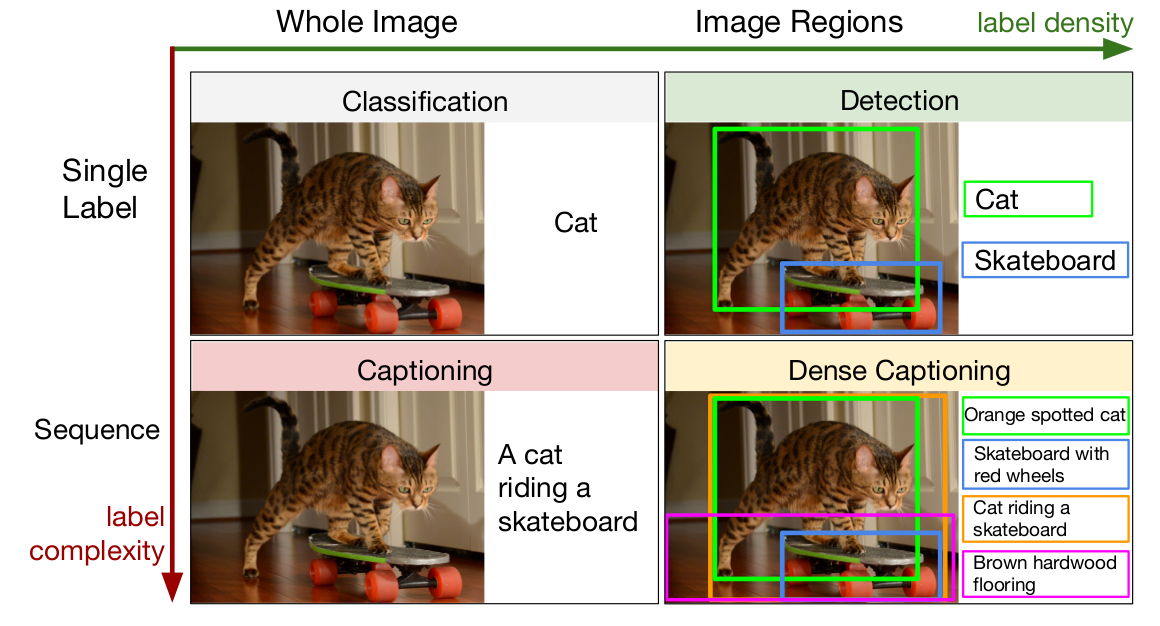
\includegraphics[scale=0.22]{data/dense-image-captioning.png}
\end{frame}
}

{%
\setbeamertemplate{frame footer}{Image: \cite{DBLP:journals/corr/KrishnaHRLN17}}
\begin{frame}[fragile]{Dense-captioning events in videos}
        \center
        \hspace*{1cm}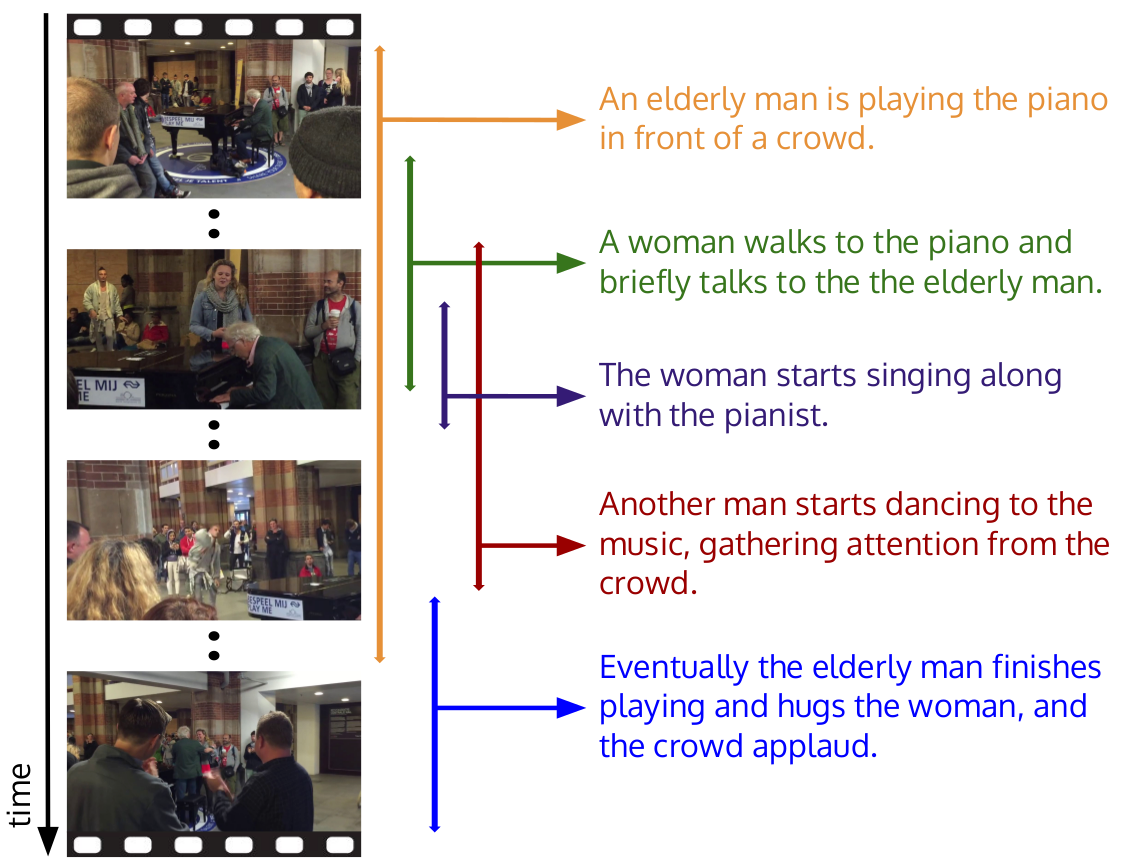
\includegraphics[scale=0.22]{data/dense-captioning-video.png}
\end{frame}
}

{%
\setbeamertemplate{frame footer}{Image: \cite{DBLP:journals/corr/KrishnaHRLN17}}
\begin{frame}[fragile]{Dense-captioning events in videos: model}
        \center
        \hspace*{-0.25cm}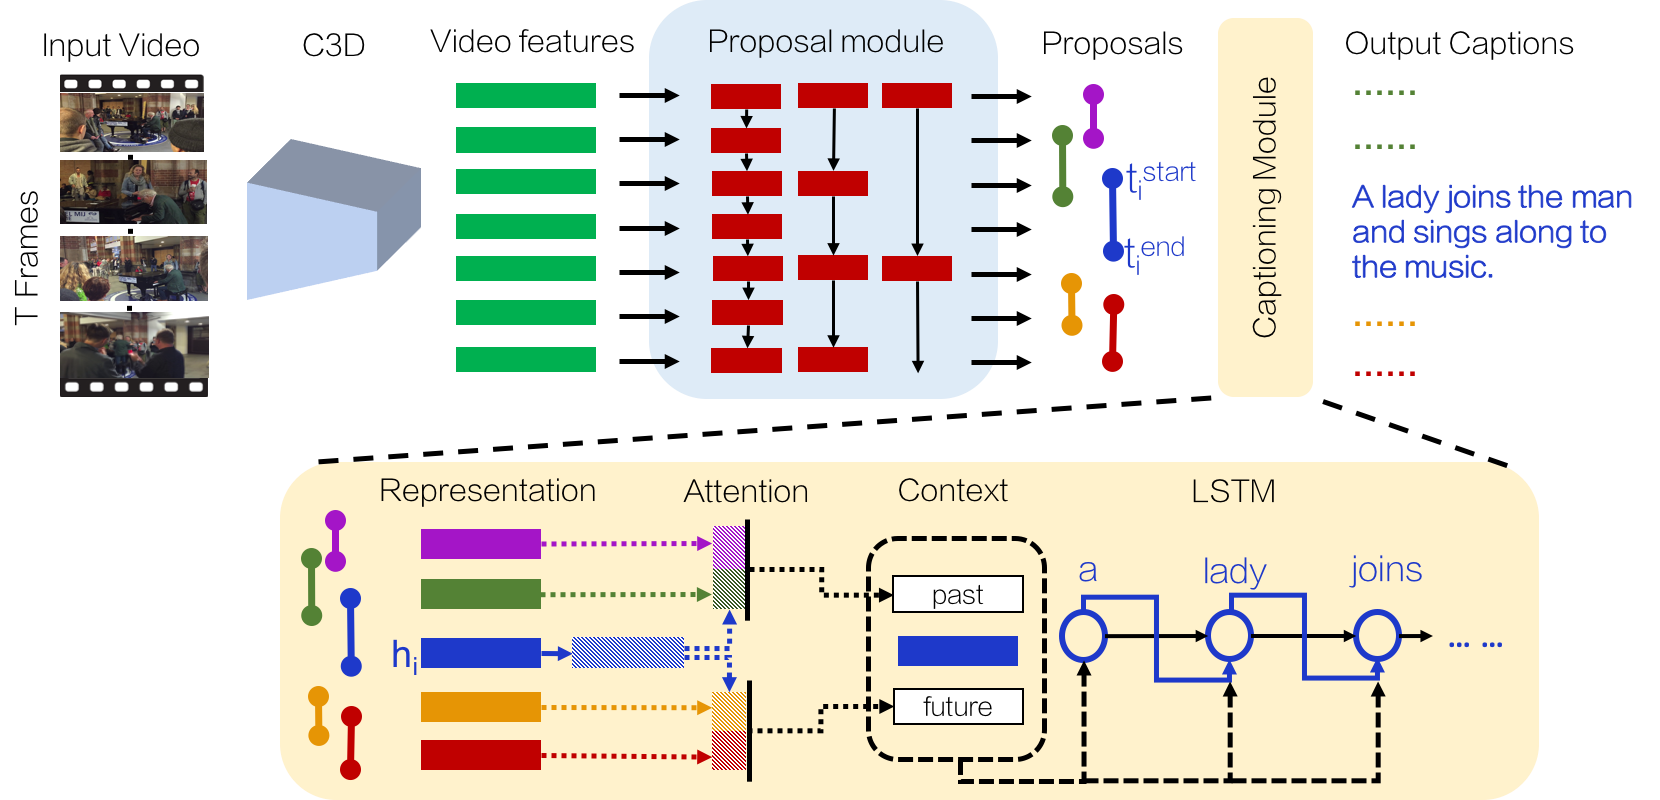
\includegraphics[scale=0.2]{data/dense-captioning-video-architecture.png}
\end{frame}
}

{%
\setbeamertemplate{frame footer}{Image: \cite{DBLP:journals/corr/KrishnaHRLN17}}
\begin{frame}[fragile]{Dense-captioning events in videos: example}
        \center
        \hspace*{0.5cm}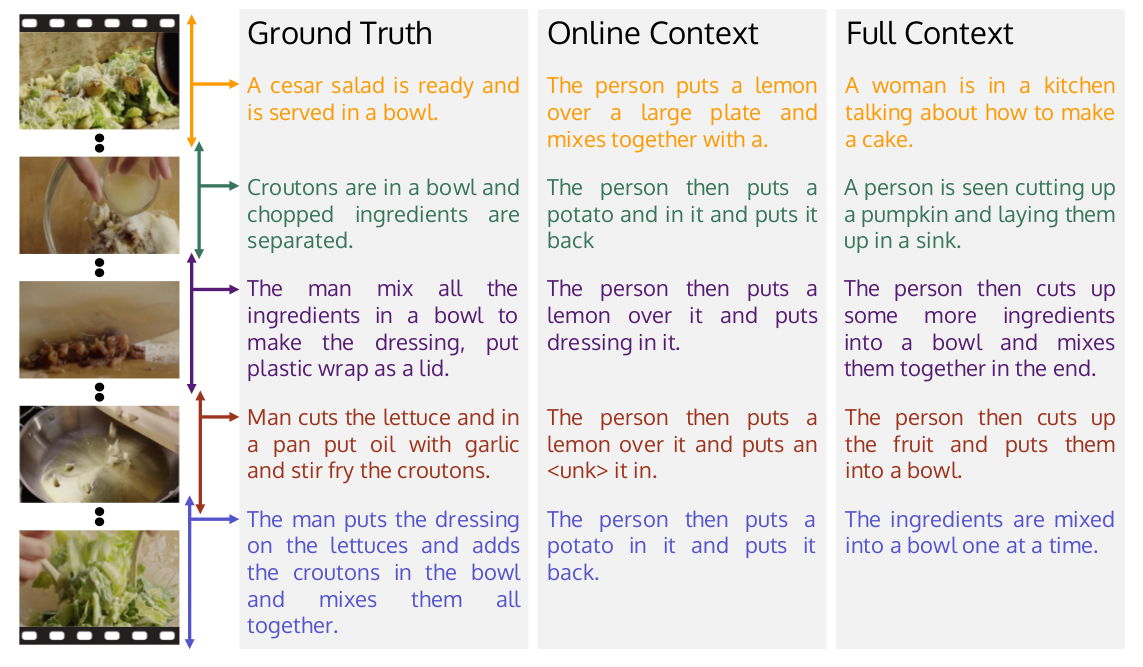
\includegraphics[scale=0.25]{data/dense-captioning-video-example.png}
\end{frame}
}

\section{Conclusions}

\begin{frame}[fragile]{Conclusions}
        \begin{itemize}[<+- | alert@+>]
                \item Current model architectures in video understanding extend
                        successful ideas from static image tasks.

                \item Optical flow significantly improves performance on video
                        understanding tasks, compared to no optical flow.

                \item Improvement over baseline static image object detection
                        is possible using Tubelet Proposal Networks.

                \item Video captioning models are able to use past and future
                        context to improve the quality of their captions.
        \end{itemize}
\end{frame}

% \section{Other image and video understanding tasks}

% \section{Leveraging the sheer volume of video data with unsupervised learning}

\begin{frame}[standout]
        Questions?
\end{frame}

\appendix

\begin{frame}[fragile]{3D two-stream nets}
        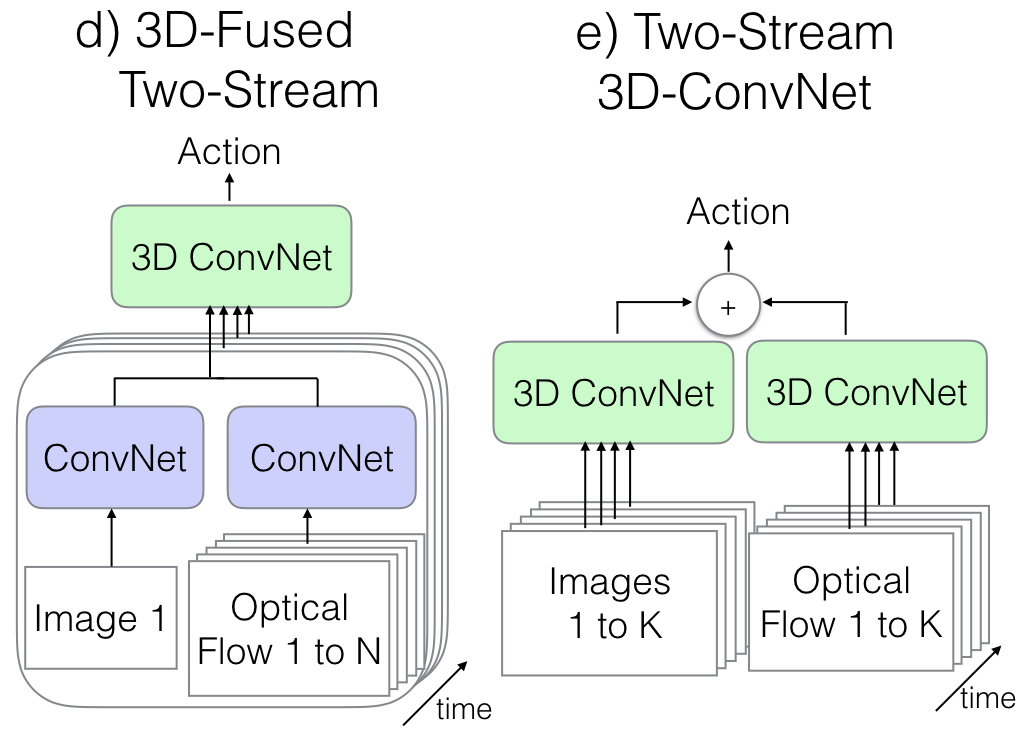
\includegraphics[scale=0.3]{data/two-stream-3d.png}
\end{frame}

\begin{frame}[allowframebreaks]{References}
        \bibliography{video-in-ml}
        \bibliographystyle{apalike}
\end{frame}

\end{document}
